\chapter{Inestabilidad en la señal de reloj}

Un sistema de sincronización debe proveer de una noción de tiempo común en el 
entorno de la red de comunicaciones en que se encuentra. La manera que tiene 
cada uno de los nodos que forman dicha red de medir el tiempo es mediante el 
conteo de los ciclos de su oscilador local. Una señal de reloj puede sufrir de 
perturbaciones tanto en amplitud como en fase, esto se modela mediante la 
ecuación \ref*{eq:clocksignal}.

\begin{equation}\label{eq:clocksignal}
x(t) = A(1+m(t))sin(\omega t + \phi (t))
\end{equation}

Para el caso de los sistemas digitales, como es el caso de \gls{wr}, podemos 
simplificar la primera componente del modelo debido a que la amplitud de la 
señal está restringida y controlada por las puertas digitales empleadas en los 
circuitos utilizados por ejemplo en una \gls{fpga}. Por tanto nos queda la 
inestabilidad en fase, fenómeno que tiene una gran repercusión sobre el 
rendimiento del sistema de recuperación y generación de reloj utilizado en WR. 
¿Por qué? Teniendo en cuenta un escenario de distribución de tiempo tipo WR, 
cada nodo compensa su reloj para seguir al del maestro. Sin embargo, la red se 
estructura por capas, lo que supone que para un nodo intermedio, la señal que 
recupera no proviene directamente del maestro, si no que puede haber pasado por 
varios niveles antes de llegar a él. El proceso de sincronización en cada nodo 
añade una pequeña componente de ruido a la señal propagada, fruto de múltiples 
fuentes de perturbación como ruido electromagnético inherente al propio 
circuito del dispositivo, ruido de otros equipos cercanos o alteraciones en la 
conductividad de los materiales por motivo de cambios de temperatura, entre 
otros. Esto supone que la calidad de la sincronización se va degradando con 
cada nuevo salto en la red, llegando incluso a imposibilitar la sincronización 
en redes con muchos nodos en cascada.

Realizar una correcta caracterización del perfil de ruido en el caso de los 
dispositivos WR es algo fundamental a la hora de realizar un análisis de las 
fuentes de perturbaciones que afectan de manera directa a la calidad de la 
sincronización. Los modelos matemáticos permiten tener una idea general del 
comportamiento que tendrá el sistema, pero es necesario disponer de equipo de 
laboratorio para realizar medidas de gran precisión a fin de caracterizar 
correctamente las fuentes de ruido.

En los siguientes apartados se introducen algunos términos clave para entender 
los aspectos relacionados con las perturbaciones en un sistema WR, y en los 
capítulos \ref{cap:cadena} y \ref{cap:reloj} se incluyen los resultados 
experimentales de la caracterización de los equipos utilizados y también 
resultados de las pruebas de rendimiento realizadas.

\section{Ruido de fase y \textit{jitter}}

Ya se ha mencionado que, como todo sistema en la vida real, el sistema de 
recuperación de reloj puede ser sufrir pequeñas perturbaciones ocasionando 
pequeños cambios en la frecuencia de oscilación de una fuente de reloj y 
también en la fase. El nombre que recibe este fenómeno en la literatura de 
electrónica digital es \textit{jitter}, y no es más que lo dicho anteriormente, 
la desviación de una señal con respecto a la ideal. La Figura \ref{fig:jitter} 
muestra este fenómeno de manera gráfica. La representación espectral de las 
variaciones temporales en una señal periódica es lo que se conoce como ruido de 
fase. Este tipo de representación permite un análisis mucho más detallado del 
ruido del sistema ya que permite diferenciar las distintas componentes que se 
integran finalmente ocasionado las pequeñas desviaciones en fase que se 
observan al medir el \textit{jitter}. La expresión matemática 
\ref{eq:parseval}, correspondiente al teorema de Parseval \cite{oppenheim96},
\begin{equation}\label{eq:parseval}
\int_{-\infty}^{+\infty} | \phi (t) |^2 dt = 
\int_{-\infty}^{+\infty} | \Phi (t) |^2 df
\end{equation}
 demuestra que es equivalente trabajar en el dominio del tiempo (denotado por 
 $\phi (t)$) que en el de la frecuencia ($\Phi (t)$), lo que permite trabajar 
 en uno u otro dominio dependiendo del tipo de análisis de ruido.



\begin{figure}
	\centering
	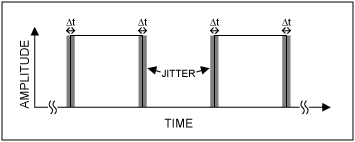
\includegraphics[width=0.5\linewidth]{imagenes/jitter}
	\caption[Ilustración del fenómeno conocido como \textit{jitter}]{En la 
	figura se muestra uan señal digital periódica que presenta pequeñas 
	variaciones en fase. Estas ligeras perturbaciones se conocen como 
	\textit{jitter} y son un efecto no deseado en las señales digitales que 
	provocan funcionamientos erróneos en los sistemas.}
	\label{fig:jitter}
\end{figure}


Dependiendo del tipo de análisis realizado y sobre todo de 
la fuente de ruido que se pretenda caracterizar, será más adecuado trabajar en 
unos casos en el dominio de la frecuencia o en el del tiempo. Sin embargo no 
siempre es posible hacerlo, dado que los aparatos necesarios para muchos de 
estos análisis son bastante caros y es complicado disponer de ellos en el 
laboratorio. \incomment{con esto cubro una posible pregunta para los resultados 
de la cadena de por qué se tomaron con el osciloscopio y no con otra cosa} El 
problema que tiene medir ruido de fase en el dominio del tiempo 
(\textit{jitter}) es el caracter no estacionario del valor RMS del mismo, que 
va creciendo con forme se aumenta el tiempo de medición.

\begin{figure}
	\centering
	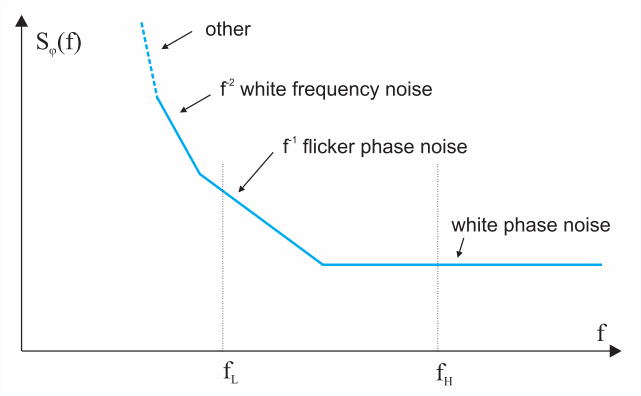
\includegraphics[width=0.7\linewidth]{imagenes/psd_noise}
	\caption[Tipos de ruido en la curva PSD para un XO.]{Clasificación del tipo 
	de ruido según la pendiente de la curva PSD para el ruido de fase de un 
	oscilador}
	\label{fig:psdnoise}
\end{figure}

La entidad IEEE define el término \textit{phase noise} \cite{ieeephysdefs} como 
la mitad 
de la inestabilidad en fase. Donde la inestabilidad en fase ( $S_{\Phi} (f)$ ) 
hace referencia a la densidad espectral de la desviación en fase de la señal. 
Una señal ideal en un oscilador generaría una señal sinusoidal pura, es decir, 
toda la potencia de la señal estaría concentrada en una única frecuencia. Sin 
embargo, esto no sucede en un oscilador real, los cuales tienen componentes de 
ruido moduladas en fase. Típicamente este tipo de medidas se expresa en dBc/Hz, 
indicando la potencia de manera relativa a la frecuencia portadora con un ancho 
de banda de 1Hz. Se utilizan varios desplazamientos con respecto a la 
frecuencia portadora de forma que se puede analizar como afecta el ruido a las 
frecuencias adyacentes a la portadora.

La Figura \ref{fig:psdnoise} muestra los distintos tipos de ruido que se 
identifican por la pendiente de la curva PSD en una doble escala logarítmica. 
En el eje de ordenadas se mide la potencia relativa a la señal portadora en dB, 
y en las abcisas la frecuencia de desplazamiento con respecto a la frecuencia 
portadora. \incomment{si hay tiempo hablar un poco del white noise y otros}

Para obtener este tipo de medidas se necesita equipo bastante caro y preciso. 
Recientemente se ha adquirido en el laboratorio del grupo de sincronización de 
la UGR un medidor de ruido de fase (ver \ref{cap:herram}) que ha posibilitado 
realizar un estudio mucho más detallado que si sólo se hubiese utilizado un 
osciloscopio convencional. Sin embargo, en las primeras fases de este proyecto 
no se contaba con dicho material por lo que se realizan las medidas que fueron 
posibles en ese momento.

\incomment{si hay un poco de tiempo mencionar ADEV y demás tipos y explicar 
rápidamente}

Para cerrar este capítulo me gustaría mencionar la diferencia entre el término 
exactitud (\textit{accuracy} en la literatura) y el de precisión 
(\textit{precision}) dado que se suelen confundir bastante entre ellos sobre 
todo con motivo de la traducción de la literatura existente y es importante 
tener clara la diferencia en el ámbito de WR. La exactitud de la sincronización 
hace referencia a la diferencia que podemos medir entre el evento generado por 
una señal del maestro, el PPS o un flanco de subida del reloj de referencia, y 
la del esclavo. Si se trabaja en el dominio del tiempo está diferencia se 
expresa en segundos y en concreto, WR, lo que consigue es que dicha diferencia 
sea menor al nanosegundo. Por otra parte hay que determinar la variación que 
sufre dicha diferencia por motivo del \text{jitter} en las señales utilizadas 
para realizar tal medida. Esto es lo que se denomina precisión, y mide la 
estabilidad de la señal generada. El objetivo de WR es que se mantenga en el 
orden del picosegundo, lo que quiere decir que la variación en la señal 
generada por el dispositivo con respecto a la ideal esté en ese orden de 
magnitud. Por tanto la estabilidad mide la evolución de la diferencia entre las 
señales entre equipos sincronizados en función de variables como el tiempo o la 
temperatura, y la precisión es una medida de la desviación de dicho valor.

